\documentclass[12pt letter]{report}
\input{../template/preamble}
\input{../template/macros}
\input{../template/letterfonts}

\usepackage{parskip}
\usepackage{booktabs}
\usetikzlibrary{arrows, positioning, shapes.gates.logic.US, circuits.logic.US, shapes.misc, automata}

\tikzset{
->, % makes the edges directed
% >=stealth’, % makes the arrow heads bold
node distance=3cm, % specifies the minimum distance between two nodes. Change if necessary.
every state/.style={thick, fill=gray!10}, % sets the properties for each ’state’ node
initial text=$ $, % sets the text that appears on the start arrow
}
\title{\Huge{Lab 5}}
\author{\huge{Madiba Hudson-Quansah}}
\date{}


\begin{document}
\maketitle
\newpage

\section*{Part 5: Analysis of Sequential Circuits}
\qs{}{
  Provide the state table for the sequential circuit.
  \begin{align*}
    A \left( t + 1 \right) & = \overline{x}y + xA \\
    B \left( t + 1 \right) & = \overline{x}B + xA \\
    z = B
  \end{align*}
}

\sol{
  \begin{table}[h!]
    \begin{center}
      \begin{tabular}{*{7}{wc{7mm}}} \toprule
        \multicolumn{2}{c}{Current State} &
        \multicolumn{2}{c}{Input}         &
        \multicolumn{2}{c}{Next State}    &
        \multicolumn{1}{c}{Output}                                            \\

        \cmidrule(lr){1-4}\cmidrule(lr){5-7}
        $A$                               & $B$ & $x$ & $y$ & $A$ & $B$ & $z$ \\
        \midrule

        0                                 & 0   & 0   & 0   & 0   & 0   & 0   \\
        0                                 & 0   & 0   & 1   & 1   & 0   & 0   \\
        0                                 & 0   & 1   & 0   & 0   & 0   & 0   \\
        0                                 & 0   & 1   & 1   & 0   & 0   & 0   \\

        0                                 & 1   & 0   & 0   & 0   & 1   & 1   \\
        0                                 & 1   & 0   & 1   & 1   & 1   & 1   \\
        0                                 & 1   & 1   & 0   & 0   & 0   & 1   \\
        0                                 & 1   & 1   & 1   & 0   & 0   & 1   \\

        1                                 & 0   & 0   & 0   & 0   & 0   & 0   \\
        1                                 & 0   & 0   & 1   & 1   & 0   & 0   \\
        1                                 & 0   & 1   & 0   & 1   & 1   & 0   \\
        1                                 & 0   & 1   & 1   & 1   & 1   & 0   \\

        1                                 & 1   & 0   & 0   & 0   & 1   & 1   \\
        1                                 & 1   & 0   & 1   & 1   & 1   & 1   \\
        1                                 & 1   & 1   & 0   & 1   & 1   & 1   \\
        1                                 & 1   & 1   & 1   & 1   & 1   & 1   \\

        \midrule
        \bottomrule
      \end{tabular}
    \end{center}
  \end{table}
}

\qs{}{
  Draw the corresponding state diagram.
}

\sol{
  \begin{figure}[H]
    \centering
    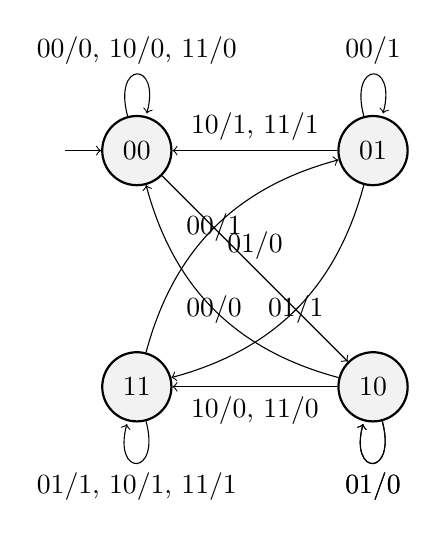
\begin{tikzpicture}
      \node[state, initial] (s0) {00};
      \node[state, right of=s0] (s1) {01};
      \node[state, below of=s1] (s2) {10};
      \node[state, below of=s0] (s3) {11};

      \draw
      (s0) edge[loop above] node{00/0, 10/0, 11/0} (s0)
      (s0) edge[above] node{01/0} (s2)
      (s1) edge[loop above] node{00/1} (s1)
      (s1) edge[bend left] node{01/1} (s3)
      (s1) edge[above] node{10/1, 11/1} (s0)
      (s2) edge[loop below] node{01/0} (s2)
      (s2) edge[loop below] node{01/0} (s2)
      (s2) edge[bend left] node{00/0} (s0)
      (s2) edge[below] node{10/0, 11/0} (s3)
      (s3) edge[loop below] node{01/1, 10/1, 11/1} (s3)
      (s3) edge[bend left] node{00/1} (s1)
      ;
    \end{tikzpicture}
  \end{figure}
}

\section*{REFLECTION QUESTIONS}

\qs{}{
  What role does the Memory Address Register (MAR) play in data transfer within a CPU, and how does it facilitate efficient memory access?
}

\sol{
  The MAR can store either the memory address from which data will be fetched, or the address to which data will be
  written and stored. This allows for efficient memory access as the lookup time for the reading or writing of data is
  reduced to a single operation due to the direct addressing of the memory location in a register which is much faster
  than if it was in memory.
}

\qs{}{
  How does using a controlled buffer with an OE pin improve the data transportation to the data bus in your ALU design?
}

\sol{
  The data bus is the primary means of data transfer between parts of the CPU. The controlled buffer controlled by the
  OE pin allows for the data to be transferred to the data bus only when needed, reducing the power consumption of the
  ALU as the buffer is only active when data is actively being outputted.
}

\qs{}{
  What challenges did you face while designing the 8-bit register and Memory Address Register? How did you resolve them?
}

\sol{
  My main challenge was intuitively understanding the bit order of the individual 1-bit register and how they came
  together to make the final output of the 8-bit register. I resolved this by dividing the 1-bit registers into two
  groups of 4 then starting the least significant bit on the right and the most significant bit on the left.
}



\end{document}
